\documentclass[11pt,aspectratio=43]{beamer}
\usepackage[utf8]{inputenc}
\usepackage{amsmath, amsfonts, amssymb, amsthm}
\usepackage[T1]{fontenc}
\usepackage{lmodern}
\usepackage{xcolor}
\usepackage{setspace}
\usepackage{booktabs}
\usepackage{multirow}
\usepackage{graphicx}
\usepackage{tikz}
% \usetikzlibrary{decorations}
\usetikzlibrary{decorations.pathreplacing}
\usepackage{ulem}
\usepackage{hyperref}
\usepackage{booktabs}
\usepackage{babel}
\usepackage{makecell}
\usepackage[para,online,flushleft]{threeparttable}
\usepackage{pdfpages}
\usepackage{tcolorbox}
\usepackage{bm}
\usepackage{appendixnumberbeamer}
\usepackage{natbib}
\usepackage{caption}
\captionsetup[figure]{labelformat=empty}% redefines the caption setup of the figures environment in the beamer class.
\usetheme[compress]{Boadilla}
\usecolortheme{default}
\useoutertheme{miniframes}
\usefonttheme[onlymath]{serif}

\newcommand{\jump}[2]{\hyperlink{#1}{\beamerbutton{#2}}}
\newcommand{\orange}[1]{\textcolor{orange}{#1}}
\newcommand{\red}[1]{\textcolor{red}{#1}}

\setbeamertemplate{itemize item}{\raisebox{0.1em}{\scalebox{0.7}{$\blacksquare$}}}
\setbeamertemplate{itemize subitem}[circle]
\setbeamertemplate{itemize subsubitem}{--}
\setbeamercolor{itemize item}{fg=black}
\setbeamercolor{itemize subitem}{fg=black}
\setbeamercolor{itemize subsubitem}{fg=black}
\setbeamercolor{item projected}{bg=darkgray,fg=white}
\definecolor{blue}{rgb}{0.2, 0.2, 0.7}
\setbeamercolor{alerted text}{fg=blue}
\setbeamertemplate{enumerate items}[circle]


\setbeamertemplate{headline}{}

%==========================================
\let\olditemize=\itemize
\let\endolditemize=\enditemize
\renewenvironment{itemize}{\olditemize \itemsep1em}{\endolditemize}
\let\oldenumerate=\enumerate
\let\endoldenumerate=\endenumerate
\renewenvironment{enumerate}{\oldenumerate \itemsep1em}{ \endoldenumerate}

\DeclareMathOperator*{\argmax}{\arg\!\max}
\DeclareMathOperator*{\E}{\mathbb{E}}
\DeclareMathOperator*{\var}{\rm Var}
\DeclareMathOperator*{\cov}{\rm Cov}

\theoremstyle{definition}
\newtheorem{assume}{Assumption}
\newtheorem{lem}{Lemma}
\newtheorem{proposition}{Proposition}
\newtheorem{thm}{Theorem}
\newtheorem{corol}{Corollary}

\begin{document}
    \title[Lecture 9]{Lecture 9 \\ Social Planner's Problem}
    \author[Hui-Jun Chen]{Hui-Jun Chen}
    \institute[OSU]{The Ohio State University}
    % \date{\today}
    \date{\today}
    \setbeamertemplate{navigation symbols}{}
    \setstretch{1.2}

%-------------------------------------------------------
{
%	\usebackgroundtemplate{\includegraphics[width=1\paperwidth]{../EveningSky_cropped_edit43_bright.jpg}}
    \begin{frame}
% \vspace{3em}
        \centering
%		{\footnotesize 	ECON 4002 Intermediate Macroeconomic Theory}
        \maketitle
% \vspace{-1.5em}
% \centering
% \includegraphics[width=0.55\linewidth]{Pictures/houses.jpeg}


    \end{frame}
}

% -------------------------------------------
\setbeamertemplate{headline}
{
\setbeamercolor{section in head/foot}{fg=black, bg=white}
\vskip1em \tiny \insertsectionnavigationhorizontal{1\paperwidth}{\hspace{0.50\paperwidth}}{}
}
%------------------------------------------

\begin{frame}{Overview}
\label{slide:Overview}
    After constructing both \alert{consumers'} and \alert{firms'} problem, we start to bring them together in \alert{one-period model}:
    \begin{itemize}
        \item Lecture 8: \alert{competitive equilibrium} (CE)
        \begin{itemize}
            \item each agent solve their problems individually
            \item aggregate decision determines ``prices'' (wage, rent, etc.)
        \end{itemize}
        \item Lecture 9: \alert{social planer's problem} (SPP)
        \begin{itemize}
            \item imaginary and benevolent social planner determines the allocation
            \item should be the most efficient outcome
        \end{itemize}
        \item Lecture 10: CE and SPP examples
    \end{itemize}
\end{frame}

\begin{frame}{What is Social Planner?}
\label{slide:What_is_Social_Planner_}
\begin{itemize}
    \item \alert{Benevolent dictator} whose goal is to maximize \alert{social welfare} given \alert{technological constraint}
    \item \textbf{Social welfare}: joint ``happiness'' of every agent in this economy
    \begin{itemize}
        \item \alert{consumer}: tangency between IC and budget line in $ ( C, l ) $-plane
        \item \alert{firm}: $ Y = z F( K, N ) = z F( K, h-l ) $
        \begin{itemize}
            \item labor market clearing: $ N = N^{s} = N^{d} $
            \item consistent with consumer behavior: $ N = h - l $
        \end{itemize}
        \item \alert{government}: income-expenditure identity, $ C = Y - G $
        \begin{itemize}
            \item government is not necessary the social planner! (also one of the agents)
        \end{itemize}
    \end{itemize}
    \item \textbf{Technological constraint}: production possibility frontier
\end{itemize}
\end{frame}

\section{PPF}
\label{sec:PPF}

\begin{frame}{Production Possibility Frontier (PPF)}
\label{slide:Production_Possibility_Frontier__PPF_}
\begin{columns}
    \begin{column}{0.5\textwidth}
        \begin{itemize}
            \item \textbf{Def}: technological possibilities for the whole economy
            %
            \begin{equation}
            \label{eq:PPF}
                C = z F( K, h-l ) - G
            \end{equation}
            %
            \item \textbf{Marginal rate of transformation} (MRT): rate to transform leisure to consumption (through work)
            %
            \begin{equation}
            \label{eq:MRT}
                \begin{split}
                    MRT_{l, C}
                        & = z D_{N} F( K, N )
                    \\
                        & = MPN
                    \\
                \end{split}
            \end{equation}
            %
        \end{itemize}
    \end{column}
    \begin{column}{0.5\textwidth}
        \begin{figure}
            \caption{\scriptsize Figure 5.2 The Production Function and the Production Possibilities Frontier}
            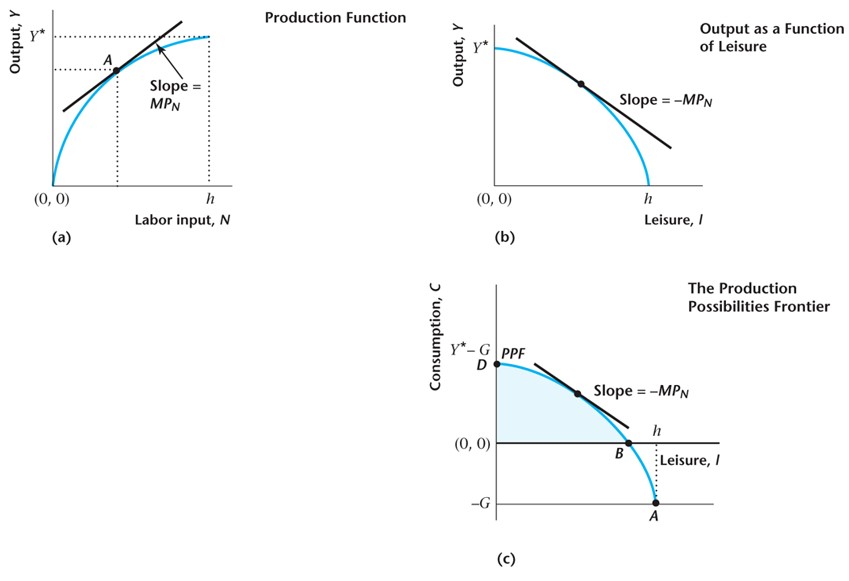
\includegraphics[width=\textwidth]{./figures/Figure5_2.jpg}
        \end{figure}
    \end{column}
\end{columns}
\end{frame}

\begin{frame}{Competitive Equilibrium: Graphcial Representation}
\label{slide:Competitive_Equilibrium__Graphcial_Representation}
    \begin{columns}
        \begin{column}{0.5\textwidth}
            \begin{figure}
                \caption{\scriptsize Figure 5.3  Competitive Equilibrium}
                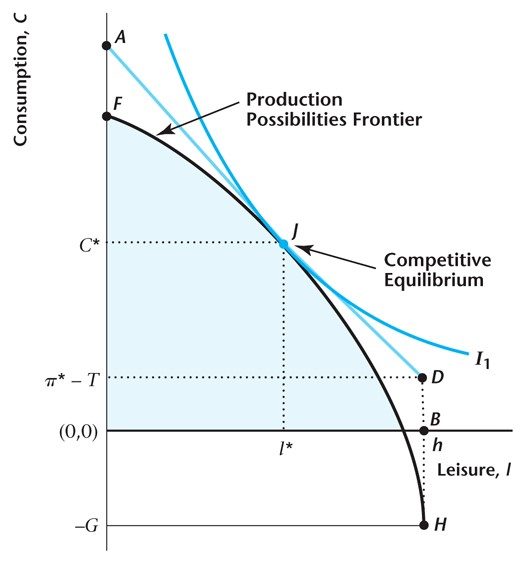
\includegraphics[width=\textwidth]{./figures/Figure5_3.jpg}
            \end{figure}
        \end{column}
        \begin{column}{0.5\textwidth}
            Combine PPF with IC:
            \begin{itemize}
                \item $\overline{AD}$: tangent to consumer's IC $ I_{1} $ and PPF $\overline{FH}$
                \item negative slope of $\overline{AD}$: equilibrium wage $ w $
                \begin{itemize}
                    \item $ \because \overline{AD}$ is budget line
                \end{itemize}
                \item Recall Lecture 8 \& last slide:
                \begin{itemize}
                    \item conumser: $ MRS_{l, C} = w $
                    \item firm: $ MPN = w $
                    \item efficiency: $ MRT_{l, C} = MPN $
                \end{itemize}
                %
                \begin{equation*}
                   MRS_{l, C} = MRT_{l, C} = MPN
                \end{equation*}
                %
            \end{itemize}
        \end{column}
    \end{columns}
\end{frame}

\section{Pareto Efficiency}
\label{sec:Pareto_Efficiency}

\begin{frame}{Concept: Pareto Improvement / Optimal}
\label{slide:Concept__Pareto_Improvement___Optimal}
    A competitive equilibrium is \textbf{Pareto optimal} or \textbf{Pareto efficient} if there is no way to \alert{rearrange production or to reallocate goods} so that \alert{someone is made better off} \red{without making someone else worse off}.
    \begin{itemize}
        \item only one consumer, so relatively straightforward
        \item but, still a powerful concept:
        \begin{itemize}
            \item free markets can produce socially efficient outcomes
            \item often easier to analyze social optimum than competitive equilibrium
        \end{itemize}
        \item caveats:
        \begin{itemize}
            \item ``efficiency'' in economics is a statement about a model
            \item very narrow: e.g. having Jeff Bezos pay for a meal for someone in need.
        \end{itemize}
    \end{itemize}
\end{frame}

\section{Social Planner}
\label{sec:Social_Planner_s_Problem}

\begin{frame}{Social Planner's Problem}
\label{slide:Social_Planner_s_Problem}
    %
    \begin{align*}
        \text{objective: consumer's utility } \quad
            & \max_{C, l, N, Y} U( C, l )
        \\
        \text{subject to} \quad
            &
        \\
        \text{agg. resource constraint} \quad
            &  C + G \le Y
        \\
        \text{production constraint} \quad
            & Y = z F( K, N )
        \\
        \text{labor constraint} \quad
            & N = h - l
    \end{align*}
    %
    \begin{itemize}
        \item \alert{What’s here}: GDP accounting, physical / technological constraints, required government spending, consumer preferences
        \item \alert{What's not}: consumer’s budget constraint, the wage rate, consumer’s / firm’s individual problems, profits, taxes
    \end{itemize}
\end{frame}

\begin{frame}{Solving Social Planner's Problem}
\label{slide:Solving_Social_Planner_s_Problem}
    We know all constraints bind, so by substituting:
    %
    \begin{equation}
    \label{eq:SPPSolve}
        \max_{l} U( z F( K, h-l ) - G, l )
    \end{equation}
    %
    \textbf{FOC}:
    %
    \begin{equation}
    \label{eq:SPPFOC}
        \begin{split}
                & D_{l} U( z F( K, h-l ) - G, l)
            \\
               = &  D_{C}U( z F( K, h-l ) - G, l ) ( z D_{N} F( K, h-l ) )
            \\
        \end{split}
    \end{equation}
    %
    \textbf{Rearrange}:
    %
    \begin{equation}
    \label{eq:SPPRearrange}
        \frac{D_{l} U( z F( K, h-l ) - G, l)}{D_{C}U( z F( K, h-l ) - G, l )} = z D_{N} F( K, h-l ) \Rightarrow MRS_{l, C}  = MRT_{l, C}
    \end{equation}
    %
    Same Result! Why?
\end{frame}

\begin{frame}{Welfare Theorem}
\label{slide:Welfare_Theorem}
    \begin{itemize}
        \item \textbf{First welfare theorem}: under centain conditions, the allocation under a competitive equilibrium is Pareto optimal
        \item \textbf{Second welfare theorem}: under certain conditions, a Pareto optimal allocation is the allocation for a competitive equilibrium.
        \item straightforward to show here (we already have!) but no always so.
        \begin{itemize}
            \item conditions not always met!
        \end{itemize}
        \item SPP and CE often alike if not identical, serves as a good benchmark
    \end{itemize}
\end{frame}

\begin{frame}{Social Planner's Problem: Graphical Representation}
\label{slide:Social_Planner_s_Problem__Graphical_Representation}
    \begin{columns}
        \begin{column}{0.5\textwidth}
            \begin{figure}
                \caption{\scriptsize Figure 5.4  Pareto Optimality}
                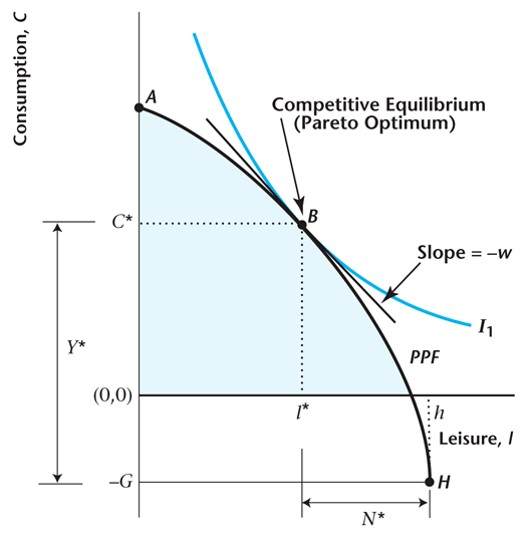
\includegraphics[width=\textwidth]{./figures/Figure5_4.jpg}
            \end{figure}
        \end{column}
        \begin{column}{0.5\textwidth}
            Apply SPP \& 2nd welfare theorme for competitive equilibrium:
            \begin{itemize}
                \item $ l^{*} $ determined by SPP at $ B $
                \item $ C^{*}, N^{*}, Y^{*} $ by plugging into constraints
                \item $ w^{*} = MPN = MRT_{l, C} = MRS_{l, C} $
            \end{itemize}
        \end{column}
    \end{columns}
\end{frame}

\begin{frame}{What Can Go Wrong? Cases when SPP $ \neq $ CE}
\label{slide:What_Can_Go_Wrong__Cases_when_SPP____neq___CE}
\begin{enumerate}
    \item Externalities: activity for which an individual does not take account of all associated costs and benefits: can be positive or negative
    \begin{itemize}
        \item example: pollution must be cleaned up, but firm doesn’t have to
    \end{itemize}
    \item Distorting taxes: lead to ``wedges'' between MRS, MP, and MRT
    \begin{itemize}
        \item example: proportional labor income tax vs lump-sum tax
    \end{itemize}
    \item Non-competitive / monopolistic behavior: firms or consumers may not be price takers
    \begin{itemize}
        \item examples: local media markets, negotiations
    \end{itemize}
\end{enumerate}
\end{frame}
\end{document}
